\documentclass[tikz,border=6pt]{standalone}
\usepackage{amsmath}
\usepackage{xcolor}
\usetikzlibrary{arrows.meta,positioning}

\definecolor{boxfill}{HTML}{DCE3EE}
\definecolor{boxstroke}{HTML}{64748B}
\definecolor{txt}{HTML}{111827}
\definecolor{dashline}{HTML}{94A3B8}

\begin{document}
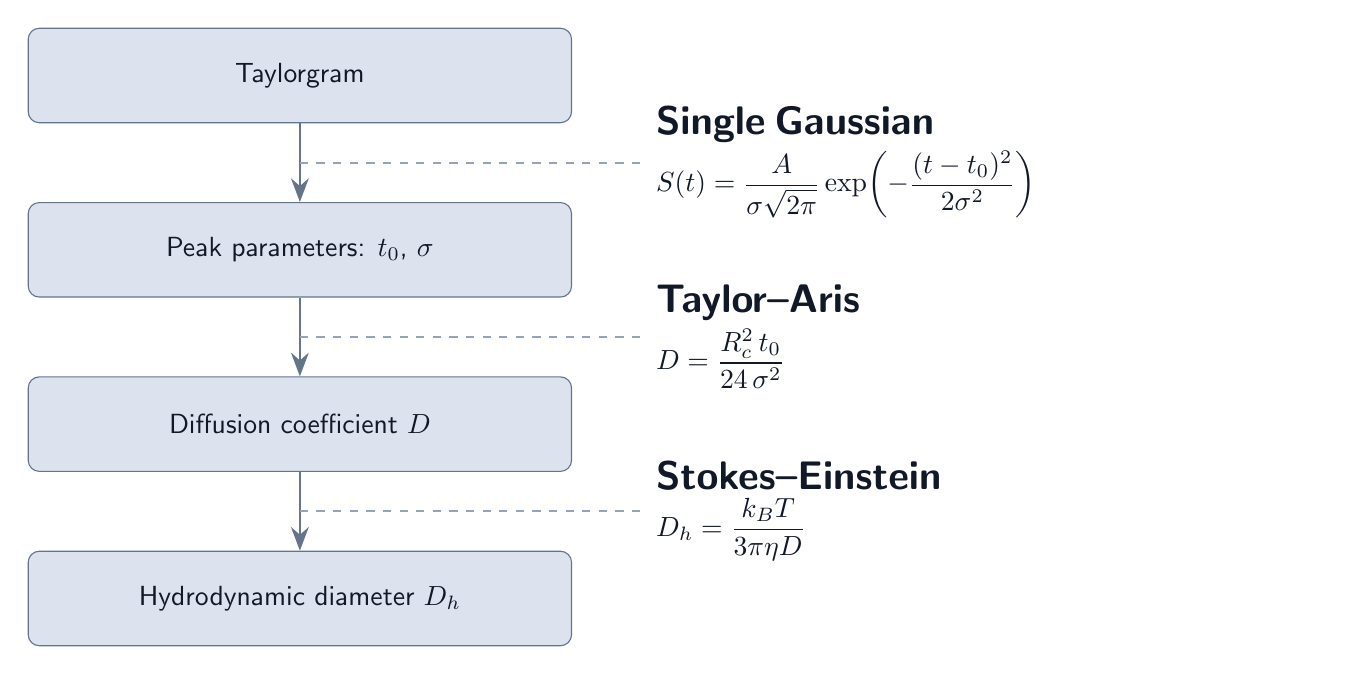
\begin{tikzpicture}[
  font=\sffamily,
  box/.style={
    draw=boxstroke,
    rounded corners=4pt,
    fill=boxfill,
    minimum width=6.9cm,
    minimum height=1.2cm,
    align=center,
    text=txt
  },
  eq/.style={
    align=left,
    text width=8.5cm,
    text=txt
  },
  arrow/.style={-{Stealth[length=3mm]}, line width=0.9pt, draw=boxstroke},
  match/.style={draw=dashline, dashed, line width=0.7pt}
]
  % Left pipeline
  \node[box] (taylor) {Taylorgram};
  \node[box, below=1.0cm of taylor] (params) {Peak parameters: $t_0$, $\sigma$};
  \node[box, below=1.0cm of params] (diff) {Diffusion coefficient $D$};
  \node[box, below=1.0cm of diff] (dh) {Hydrodynamic diameter $D_h$};

  % Main flow arrows with midpoint anchors (match thesis slide layout)
  \draw[arrow] (taylor) -- (params) coordinate[midway] (mid1);
  \draw[arrow] (params) -- (diff) coordinate[midway] (mid2);
  \draw[arrow] (diff) -- (dh) coordinate[midway] (mid3);

  % Right equations
  \node[eq, right=4.4cm of mid1] (eqg) {
    {\Large\bfseries Single Gaussian}\\[0.2em]
    $\displaystyle S(t)=\frac{A}{\sigma\sqrt{2\pi}}
      \exp\!\left(-\frac{(t-t_0)^2}{2\sigma^2}\right)$
  };

  \node[eq, right=4.4cm of mid2] (eqt) {
    {\Large\bfseries Taylor--Aris}\\[0.2em]
    $\displaystyle D=\frac{R_c^{2}\,t_0}{24\,\sigma^{2}}$
  };

  \node[eq, right=4.4cm of mid3] (eqs) {
    {\Large\bfseries Stokes--Einstein}\\[0.2em]
    $\displaystyle D_h=\frac{k_BT}{3\pi\eta D}$
  };

  % Dashed mapping lines
  \draw[match] (mid1) -- (eqg.west);
  \draw[match] (mid2) -- (eqt.west);
  \draw[match] (mid3) -- (eqs.west);
\end{tikzpicture}
\end{document}
